

\chapter{\uppercase{Existing Works}}

Existing literature proposing DNS systems for Tor is fairly sparse, though some ideas have been put forward.

\section{Clearnet DNS}

The Internet Domain Name Service (DNS) is a hierarchical distributed naming system for computers connected to the Internet. It links two principal Internet namespaces, Internet Protocol (IP) addresses and domain names, and translates one to the other. IP addresses specify the location of a computer or device on a network and domain names identify that resource. Domain names also serve as an abstraction layer so that devices can be moved to a different physical location or to a different IP address without loss of functionality. In contrast to IP addresses, domain names are human-meaningful and easily memorized, so DNS is a crucial component to the usability of the Internet.

Domain names on the Internet consist of a sequence of labels, delimited by dotes. The right-most label is the top-level domain (TLD) and can be used to classify the Internet resource by country or by organization type, although generic TLDs are more common. One or more subdomains follow the TLD. Each label can consist of up to 63 characters and the domain names can be up to 253 characters.



\section{Namecoin}

% TODO: expand: I spend six pages on Tor + hidden services, I should spend six pages on BTC + Namecoin, and two on DNS
% question: I'm aiming for 50 pages, and it looks I'll be burning 14 or 15 on introductions. Is that all right? If not, reduce to 5 + 5 + 1

Bitcoin is a decentralized peer-to-peer digital cryptocurrency, created by pseudonymous developer Satoshi Nakamoto in 2008. Ownership of Bitcoins consists of holding a private ECDSA key, and a transfer is a transmission of Bitcoins from one key to another. All transactions are recorded on a public ledger, called a blockchain, a data structure whose integrity is ensured through computational power but publically verifiable. Bitcoins are generated computationally at a fixed rate by \textit{miners} in a process that also secures the blockchain. Although Bitcoin received limited attention in the first two years of its life, it has since grown significantly since then, with approximately 70,000 daily transactions as of the time of this writing. Bitcoin's growth has led to the creation of many alternative cryptocurrencies, and its popularity has influenced financial discussions and legal controversy worldwide.

\subsection{Architecture}

A blockchain is data structure fundamental to Bitcoin, and crucial for its functionality. As a distributed decentralized system, this public ledger is Nakamoto's answer to the problem of ensuring agreement of critical data across all involved parties. The blockchain is a novel structure, and its structure guarantees integrity, chronological ordering of transactions, and the prevention of double-spending of Bitcoins. The blockchain consists of blocks of data that are held together by proof-of-work, a cryptographic puzzle whose solution is provably hard to find but trivial to verify. Bitcoin's proof-of-work is based on Adam Back's Hashcash scheme: that is, find a nonce such that the hash of this nonce and some data produces a result that begins with a certain number of zero bits. In Bitcoin's case this is stated as finding a nonce that when passed through two rounds of SHA256 ($ \textrm{SHA}256^{{2}} $) produces a value less than or equal to a target $ T $. This requires a party to perform on average $ \frac{1}{Pr[H \leq T]} = \frac{2 ^ {{256}}}{T} $ amount of computations, but it is easy to verify that $ \textrm{SHA}256^{{2}}(\textrm{msg} || n) \leq T $. Nodes in the Bitcoin network collectively agree to use the blockchain with the highest accumulation of computational effort, so an adversary seeking to modify the structure would need to recompute the proof-of-work for all previous blocks as well as out-perform the network, which is currently considered infeasible.\cite{Okupski2014}

Each block in the blockchain consists of a header and a payload. The header contains a hash of the previous block's header, the root hash of the Merkle tree built from the transactions in this block, a timestamp, a target $ T $, and a nonce. The block payload consists of a list of transactions. The root node of the Merkle tree ensures the integrity of the transaction vector: verifying that a given transaction is contained in the tree takes $ log(n) $ hashes, and a Merkle tree can be built $ n * log(n) $ time, ensuring that all transactions are accounted for. The hash of the previous block in the header ensures that blocks are ordered chronologically, and the Merkle root hash ensures that the transactions contained in each block are order chronologically as well. The target $ T $ changes every 2016 blocks in response to the speed at which the proof-of-work is solved such that Bitcoin miners take two weeks to generate 2016 blocks, or one block every 10 minutes. The $ \textrm{SHA}256^{{2}} $ proof-of-work provides integrity of the data structure, and secp256k1 ECDSA key are used to prove ownership of coins.\cite{Okupski2014}

\begin{figure}[htbp]
	\centering
	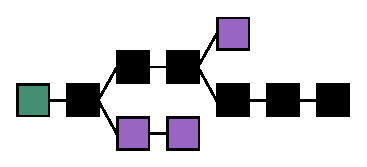
\includegraphics[width=0.6\textwidth]{images/Blockchain-2.eps}
	\caption{A sample blockchain.}
	\label{fig:figure6}
\end{figure}

\begin{figure}[htbp]
	\centering
	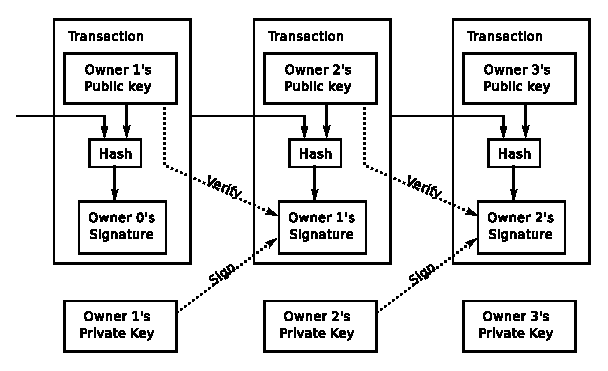
\includegraphics[width=0.6\textwidth]{images/bitcoin_transaction.eps}
	\caption{Three traditional Bitcoin transactions.}
	\label{fig:figure7}
\end{figure}

In the possibility that multiple nodes solve the proof-of-work and generate a new block simultaneously, the block becomes orphaned, the transactions recycled, and the blockchain follows the longest path from the genesis node to the latest block. Each transaction contains the public of the recipient, the ECDSA digital signature of the transaction from the sender, and the hash of the originating transaction. In this way, the digital signatures and proof-of-work in the blockchain can be traced back to the origin and forwards indefinitely. %In practice transactions can contain multiple input and outputs.

In recent years, systems have been developed that have shown Zooko's Triangle to be false. One prominent example is Namecoin, a naming system which uses a Bitcoin-like blockchain to store name-value pairs. Human-meaningful names can be embedded in the blockchain, which is distributed by nature. The uniqueness of the names is ensured by the Namecoin network and can be verified with anyone holding the blockchain. However, Tor developers have been wary of using Namecoin to store domain names for Tor hidden services. It is also impractical to require all Tor clients to download the entire blockchain before being able to use a hidden service DNS system, and there are inherent security challenges involved with querying servers or the Namecoin network for a registration without being able to use a complete blockchain to verify it. Therefore, another solution is needed.

Namecoin is a decentralized information registration and transfer system based on Bitcoin. It was the first software fork of Bitcoin and was introduced in April 2011. It uses its own blockchain and can hold name-value pairs in the blockchain attached to coins. While Bitcoin is primarily focused on supporting a currency, Namecoin aims to be a general key-value store, capable of holding cryptographic keys, DNS registrations, or other arbitrary data. It is most commonly used as a secure and censorship-resistance replacement for clearnet DNS. In 2014, Namecoin was recognized by ICANN is the most well-known example of a PKI and DNS system with an emphasis of distributed control and privacy, a growing trend in light of the revelations about the US Government by Edward Snowden. %https://www.icann.org/en/system/files/files/report-21feb14-en.pdf

\subsection{Names}

Although it inheriting Bitcoin's existing infrastructure, Namecoin added several transaction types specifically for registering and processing names, along with two new rules: names in the blockchain expire after 36,000 blocks unless renewed by the owner and no two unexpired names can be identical. These rules are enforced in the blockchain by Namecoin nodes and anyone verifying the Namecoin blockchain. Registering a name consumes 0.01 Namecoin, names can also be transferred to other owners, and they are two types: DNS and personal. The DNS type uses a new Top Level Domain (TLD) not in use by ICANN: .bit, and is used for DNS registrations. The personal name can contain arbitary data, including user information such as cryptographic keys. Like Bitcoin, Namecoin's maximum block size is one megabyte and the difficulty is set such that blocks generate every 10 minutes. Thus names expire every 250 days. 





\section{Different Encoding}

One of the most prominent is a 2011 Bachelor's thesis which outlines representing a hidden service's domain name as a series of words, rather than a base58-encoded hash.\cite{NicolussiThesis2011} However, while this scheme would improved recognition and memorability of hidden services, the words would remain random, are not chosen in advance, and do not relate to the hidden service in any meaningful way. Therefore this solution is an improvement but is not a solution. The problem remains open.